\section{評価方法と結果}
\subsection{評価方法}
報告者が担当した楽器音源について，各楽器の音確認テストと演奏テストの2つを実施した．音確認テストでは
客観評価と主観評価の両面から，演奏テストでは発音の完遂性から評価を行った．

\subsubsection{音確認テスト}
音確認テストでは，Processingによって生成される音が，各楽器の物理的特性に基づく理論的な周波数を
正確に再現できているかを検証する．客観評価では，合成音の波形を取得し，その基本周波数を測定して
目標とする音高の理論周波数と比較する．基本周波数の測定には，自己相関法およびゼロ交差法を用いた．
測定された周波数$f_\mathrm{meas}$と理論周波数$f_\mathrm{ref}$との相対誤差を次式で定義する．
\begin{equation}
  \varepsilon = \frac{|f_\mathrm{meas} - f_\mathrm{ref}|}{f_\mathrm{ref}} \times 100 \quad [\%]
\end{equation}
評価基準は，相対誤差$\varepsilon$が$\pm1.0$\,\%以内であることとした．

主観評価では，被験者に各楽器の音を提示し，「意図された楽器を正しく識別できる」および「音の減衰や
響きが自然である」の2項目について5段階（5:非常にそう思う〜1:全くそう思わない）で評価を得た．
被験者数を$N$，各被験者の評価値を$S_i$としたとき，平均評価値$S_\mathrm{avg}$を次式で定義する．
\begin{equation}
  S_\mathrm{avg} = \frac{1}{N}\sum_{i=1}^{N} S_i
\end{equation}
評価基準は，平均評価値$S_\mathrm{avg}$が4.0以上であることとした．

\subsubsection{演奏テスト}
演奏テストでは，Arduinoによる譜面配列の参照からProcessingでの発音に至るまで，実曲の演奏において
システムが正常に機能するかを検証する．複数の小節にわたる連続的な演奏を対象とし，リズムのずれや
音の欠落が発生しないかを確認する．評価指標として，正常に発音された音符数の割合を示す発音成功率
$R_\mathrm{success}$を次式で定義する．
\begin{equation}
  R_\mathrm{success} = \frac{\text{正常発音数}}{\text{全音符数}} \times 100 \quad [\%]
\end{equation}
ここで正常発音数は，譜面配列の音符情報が欠落なくProcessingへ送信され，設計通りの周波数で発音された
回数を示す．評価基準は，発音成功率$R_\mathrm{success}$が100\,\%であることとした．

\subsection{客観評価の結果}
各楽器音源の客観評価の結果を表\ref{tab:objective}に示す．また，各楽器について，実際の楽器の音の波形と
合成音の波形を取得し，比較を行った．

報告者が担当したトロンボーンでは，目標とするC3（理論周波数131.0\,Hz）に対し，測定された周波数は
131.05\,Hz，音高の誤差は$+0.3$\,centであり，誤差$\pm1.0$\,\%以内という基準を満たした．
トロンボーンの実際の音の波形を図\ref{fig:trom_real}に，合成音の波形を図\ref{fig:trom_record}に示す．
実際の波形は，基本周期ごとに鋭いピークを持つ倍音の豊かな波形を示している．合成音の波形も同様に
周期的な波形を示しており，基本周波数が再現できていることが確認できる．一方で，合成音は実際の波形に
比べて振幅が小さく，波形の細部の複雑さも少ない．これは，後述するように音源の音量が小さいこと，
および倍音構成が実際の楽器と完全には一致していないことによると考えられる．

カスタネットについては，音程を持たない打楽器であるため，周波数の誤差ではなく波形の特性で評価した．
カスタネットの実際の音の波形を図\ref{fig:cast_real}に，合成音の波形を図\ref{fig:cast_record}に示す．
実際の波形は，打撃の瞬間に振幅が最大となり，その後不規則に振動しながら急速に減衰している．
合成音の波形も，立ち上がり直後に振幅が最大となり，約20\,msで減衰する打撃音特有の波形を示した．
ピーク振幅は0.17であり，音程を持たない打撃音として妥当な波形が得られたと判断した．

また，参考として，他のメンバーが担当したピアノおよびヴァイオリンについても客観評価を行い，
いずれも理論周波数との誤差$\pm1.0$\,\%以内を満たした．さらに，すべての楽器について実曲演奏テストを
行い，全音符が欠落なく発音され，発音成功率は100\,\%であった．

\begin{table}[H]
  \centering
  \caption{楽器音源の客観評価の結果}
  \label{tab:objective}
  \begin{tabular}{lccc}
    \hline
    楽器 & 目標周波数 & 測定結果 & 判定 \\
    \hline
    ピアノ & C4（261.6\,Hz） & 261.67\,Hz（$+0.3$\,cent） & 達成 \\
    トロンボーン & C3（131.0\,Hz） & 131.05\,Hz（$+0.3$\,cent） & 達成 \\
    ヴァイオリン & C4（261.6\,Hz） & 263.15\,Hz（$+0.58$\,cent） & 達成 \\
    カスタネット & --- & 約20\,msで減衰する打撃波形 & 達成 \\
    \hline
  \end{tabular}
\end{table}

\begin{figure}[H]
  \begin{minipage}{0.5\linewidth}
    \centering
    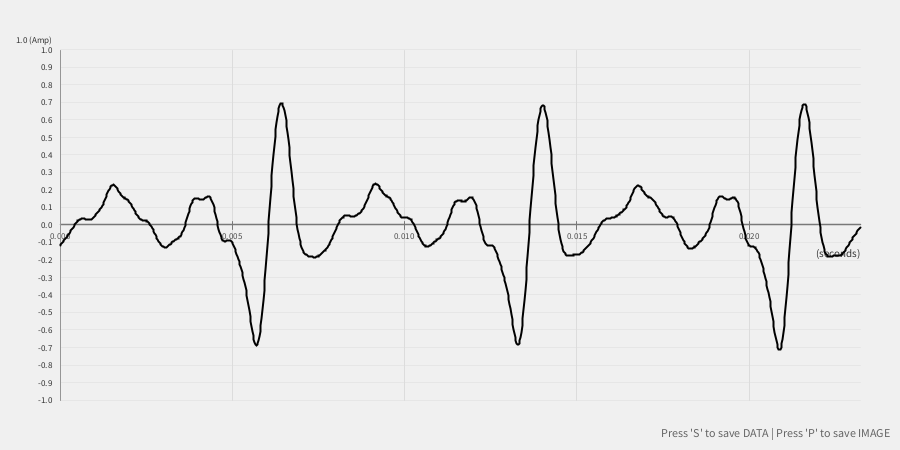
\includegraphics[width=\linewidth]{fig/trombone_real.png}
    \caption{トロンボーン（実物）の波形}
    \label{fig:trom_real}
  \end{minipage}%
  \begin{minipage}{0.5\linewidth}
    \centering
    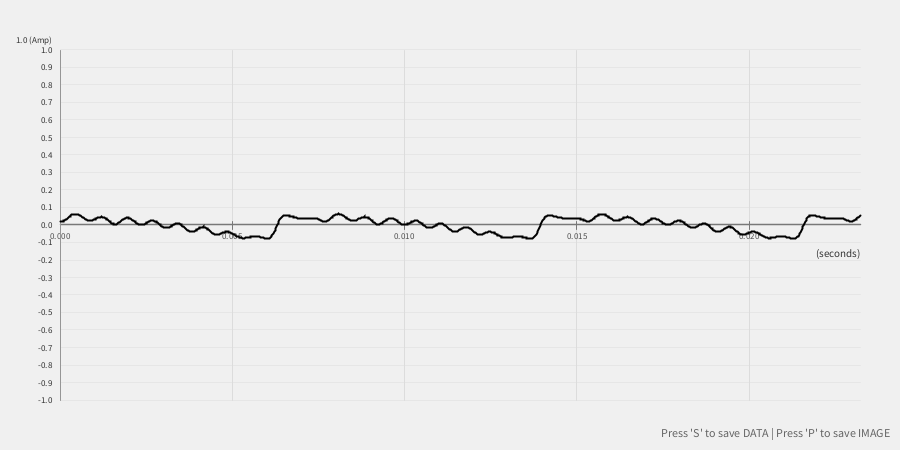
\includegraphics[width=\linewidth]{fig/trombone_record.png}
    \caption{トロンボーン（合成音）の波形}
    \label{fig:trom_record}
  \end{minipage}
\end{figure}

\begin{figure}[H]
  \begin{minipage}{0.5\linewidth}
    \centering
    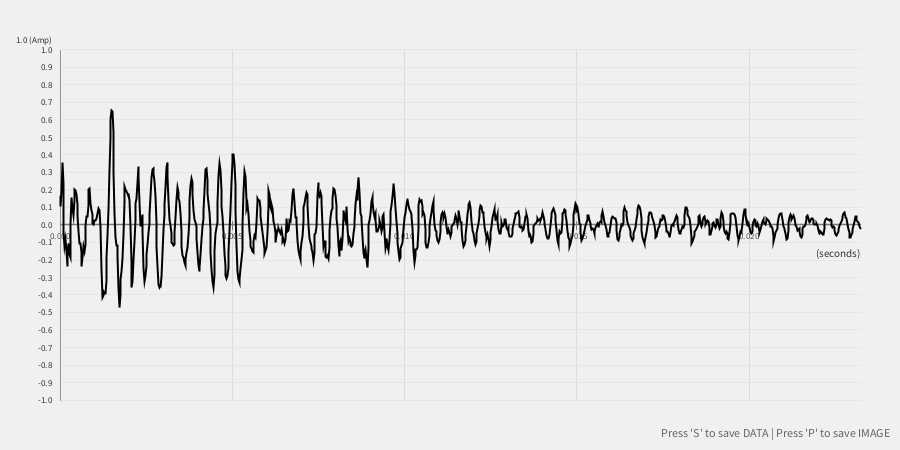
\includegraphics[width=\linewidth]{fig/castanet_real.png}
    \caption{カスタネット（実物）の波形}
    \label{fig:cast_real}
  \end{minipage}%
  \begin{minipage}{0.5\linewidth}
    \centering
    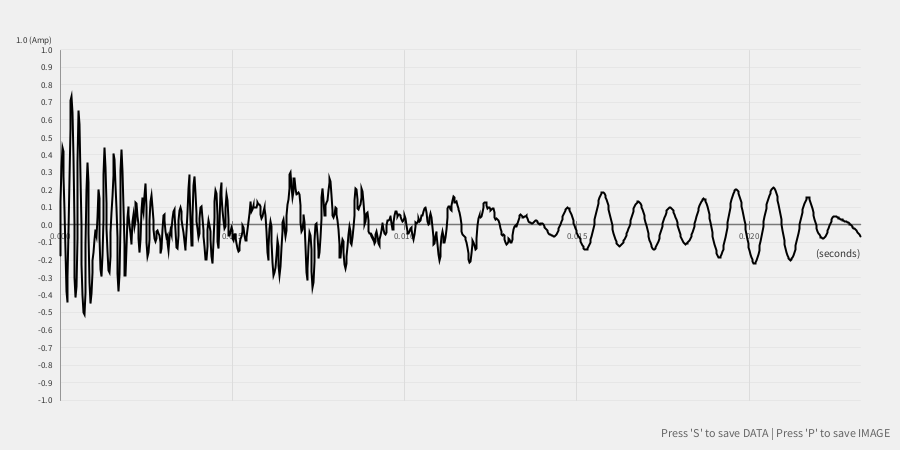
\includegraphics[width=\linewidth]{fig/castanet_record.png}
    \caption{カスタネット（合成音）の波形}
    \label{fig:cast_record}
  \end{minipage}
\end{figure}

\subsection{主観評価の結果}
32名を対象に実施したアンケートによる主観評価の結果を表\ref{tab:subjective}に示す．報告者が担当した
トロンボーンは，作成音3.88，音質3.97であり，全楽器の中で比較的高い評価を得た．カスタネットは
作成音3.44，音質3.81であった．一方で，いずれの楽器も作成音の評価は基準の4.0に達しなかった．
これは，合成音の音量が小さいことや，演奏時のサーボモータの駆動音が影響したためと考えられる．
音質については，トロンボーンをはじめ複数の楽器で3.8以上の評価が得られた．

\begin{table}[H]
  \centering
  \caption{楽器音源の主観評価の結果（$n=32$，5段階）}
  \label{tab:subjective}
  \begin{tabular}{lcc}
    \hline
    楽器 & 作成音 & 音質 \\
    \hline
    ピアノ & 3.56 & 3.97 \\
    トロンボーン & 3.88 & 3.97 \\
    ヴァイオリン & 3.06 & 3.22 \\
    カスタネット & 3.44 & 3.81 \\
    \hline
  \end{tabular}
\end{table}